%%%% Document type  %%%%
\documentclass[preprint,12pt,fleqn]{article}
 \usepackage{ragged2e}
\usepackage{authblk}  % Package for author affiliations
% \usepackage{nopageno} % no page numbers
\usepackage[rightcaption]{sidecap}

\usepackage[most]{tcolorbox}
\newtcolorbox[auto counter,number within=chapter]{definition}[1][]{
  enhanced,
  breakable,
  fonttitle=\scshape,
  title={Definition \thetcbcounter},
  #1
}

%%%% Document structure %%%%
%\usepackage{geometry}
\usepackage[verbose=true,letterpaper]{geometry}
\geometry{
%    a4paper,
%    left=30mm,
%    right=30mm,
%    top=30mm,
%    bottom=30mm,
    textheight=9in,
    textwidth=5.5in,
    top=1in,
    headheight=12pt,
    headsep=25pt,
    footskip=30pt,
   % phone  
   %a5paper,
   %width=120mm,
  %height=180mm,
}

\usepackage{lineno} % used along with \linenumbers after begin document. 
\usepackage{setspace} 
\setstretch{1.2}
\makeatletter % The following lines get rid of footer stating pre-preint to elsevier.
\def\ps@pprintTitle{%
\let\@oddhead\@empty
\let\@evenhead\@empty
\def\@oddfoot{}%
\let\@evenfoot\@oddfoot}
\makeatother
\graphicspath{ {../images/} }
\usepackage{pgf} % calculate cohort stats percentage

%%%% Bibliography   %%%%
\usepackage{natbib}
\setcitestyle{numbers,sort&compress}
\setcitestyle{sort&compress}
\usepackage{hypernat} 
    
%%%% Aesthetics     %%%%
\usepackage{microtype}
% \RequirePackage{times} % Font
\usepackage{ccaption}
\usepackage{siunitx}
\usepackage[T1]{fontenc}
\usepackage[utf8]{inputenc}
\usepackage{nameref}% this allows a reference be named, to print unnumbered references by their section name (used here for linking to Supplemental text in this case).

%%%% Paragraph Formatting %%%
\setlength{\parindent}{2em}
\setlength{\parskip}{6pt plus 2pt minus 1pt}

%%%% Supplemental labels%%%%
%Define command to start a supplemental section
%set the supplemental letter used for figures (e.g. Figure E1)
\newcommand{\beginsupplement}{%
        \setcounter{table}{0}
        \renewcommand{\thetable}{E\arabic{table}}%
        \setcounter{figure}{0}
        \renewcommand{\thefigure}{E\arabic{figure}}%
         }

%%%% Building tables%%%%
\usepackage{booktabs} % required for tables
\usepackage{rotating,tabularx} 
\newcolumntype{Z}{ >{\centering\arraybackslash}X } % defining table content layout per box
\usepackage{ltablex} % allow page break between lines in tabularx
% \usepackage{caption} \captionsetup{font=normalsize} % to set the caption size as normal even when table is tiny.
\usepackage{multirow}
\usepackage{pdflscape}

%%%% Colors %%%%
\usepackage{xcolor} 
\definecolor{natureblue}{RGB}{5,110,210}
    \usepackage[colorlinks]{hyperref} 
\AtBeginDocument{%this allows colours to chage from the defined elsearticle template.
\hypersetup{
    	colorlinks=true,
        linkcolor={natureblue},
    	citecolor={natureblue},
        filecolor=blue!50!black,
        urlcolor=cyan,
    	}}

\definecolor{kispiblack}{HTML}{333333}
\definecolor{kispidarkblue}{HTML}{023047}
\definecolor{kispidarkgreen}{HTML}{006666}
\definecolor{kispired}{HTML}{C70000}
\definecolor{kispilink}{HTML}{007DB8}%219EBC
% \color{kispi_black} %default
\definecolor{kispiblue}{HTML}{701A57}
% City sunset: https://www.color-hex.com/color-palette/40131
\definecolor{colorSUNSET1}{HTML}{eeaf61}
\definecolor{colorSUNSET2}{HTML}{fb9062}
\definecolor{colorSUNSET3}{HTML}{ee5d6c}
\definecolor{colorSUNSET4}{HTML}{ce4993}
\definecolor{colorSUNSET5}{HTML}{6a0d83}
\definecolor{natureblue}{RGB}{5,110,210}    
\usepackage{dirtree}  % Load the dirtree package


% command to use these colors and formatting; xspace for correct spacing including with punctuation marks.
\usepackage{xspace}
\newcommand{\variablesdarkgreen}[1]{\textbf{\textcolor{kispidarkgreen}{#1}}\xspace}

%%%% Fancy stuff %%%%
%\usepackage{fancyhdr}
%\pagestyle{fancy}
%\lhead{My Name}
%\chead{}
%\rhead{\thepage}
%\cfoot{} % get rid of the page number 
%\renewcommand{\headrulewidth}{0pt}
%\renewcommand{\footrulewidth}{0pt}
 
 
%\usepackage{fancyhdr}
%\usepackage{lastpage}
%\pagestyle{fancy}
%\fancyhf{}
%\rfoot{\thepage}
%\cfoot{} % get rid of the page number 
%\renewcommand{\headrulewidth}{0pt}
%\renewcommand{\footrulewidth}{0pt}

 
\usepackage{tocloft}  % Customizing the Table of Contents
\setcounter{tocdepth}{2}


%%%% Include code %%%%
% \usepackage{verbatim}

\usepackage{listings}
\lstset{
    basicstyle=\ttfamily\small,
    breaklines=true,
    postbreak=\mbox{\textcolor{red}{$\hookrightarrow$}\space}, % 
    breakatwhitespace=false,
    % frame=single,
    showstringspaces=TRUE, % Don't show spaces in strings as special characters
    tabsize=2, 
    language=sh 
}

\usepackage{fontspec}
% \setmainfont{IBM Plex Sans}
% \setmonofont{IBM Plex Mono}
% \usepackage{unicode-math}
% \setmathfont{IBM Plex Math}

%\renewcommand{\rmdefault}{ptm}
%\renewcommand{\sfdefault}{phv}


% {{\ttfamily \hyphenchar\the\font=`\-} % set hyphenation for texttt blocks

\usepackage{xpatch}
\xpatchcmd{\AC@deflist}
  {\addtolength{\leftmargin}{\labelsep}}
  {\addtolength{\leftmargin}{\labelsep}\setlength{\itemsep}{0pt}}
  {}{}
\makeatother
\usepackage[printonlyused,withpage,nohyperlinks]{acronym}
%\usepackage{acronym}
% \geometry{
% phone  
b6paper,
%width=110mm,
%height=160mm,
left=10mm,
right=10mm,
top=10mm,
%bottom=20mm,
}

\begin{document}
%\maketitle
% \linenumbers
%\raggedright

\newcounter{myboxcounter}
\newcommand{\boxlabel}[1]{%
  \refstepcounter{myboxcounter}%
  \label{#1}%
}

%\textbf{box~\ref{def:VariantOutcomesDetailed}}.
%\begin{definition}[label=def:VariantOutcomesDetailed]
%\end{definition}\\

\title{Application of qualifying variants for genomic analysis}

% target: Scientific data https://www.nature.com/sdata/author-instructions
% target: Bioinformatics https://academic.oup.com/bioinformatics/

\author[1]{Dylan Lawless\thanks{Addresses for correspondence: \href{mailto:Dylan.Lawless@uzh.ch}{Dylan.Lawless@kispi.uzh.ch}}}
\author[2]{Ali Saadat}
\author[2]{Mariam Ait Oumelloul}
\author[2]{Simon Boutry}
\author[1]{Veronika Stadler}
\author[3]{Sabine Österle}
\author[3]{Jan Armida}
\author[4]{David Haerry}
\author[5]{Sean D. Froese}
\author[2]{Jacques Fellay}
%\author[1]{Consortium Members}
\author[1]{Luregn J. Schlapbach}
\affil[1]{Department of Intensive Care and Neonatology, University Children's Hospital Zürich, University of Zürich, Switzerland.}
\affil[2]{Global Health Institute, School of Life Sciences, École Polytechnique Fédérale de Lausanne, Switzerland.}
\affil[3]{Personalized Health Informatics Group, SIB Swiss Institute of Bioinformatics, Basel, Switzerland.}
\affil[4]{Positive Council, Zürich, Switzerland}
\affil[5]{Division of Metabolism and Children’s Research Center, University Children’s Hospital Zürich, University of Zurich, Zurich, Switzerland}


\maketitle
\justify
% \tableofcontents
% \listoffigures
% \listoftables

\clearpage

\begin{abstract}
\noindent
\textbf{Motivation:} \\[1ex]
Qualifying variants (QVs) are genomic alterations selected using defined criteria within genomic processing pipelines. Although essential for both genetic research and clinical diagnostics, QVs are typically regarded as simple filters rather than dynamic, multifaceted components that influence the entire analytical workflow. Existing best practices adhere to variant classification standards and standardised workflows, yet a unified framework to integrate and optimise QVs for advanced, multi-stage applications is lacking.
\\[1ex]
\noindent
\textbf{Results:} \\[1ex]
We propose a redefinition of QVs by outlining several common QV sets and demonstrating their roles within analysis pipelines. By introducing new terminology and a standard reference model, our framework enables systematic integration and standardisation of QVs, thereby enhancing reproducibility, interpretability, and interdisciplinary communication. A validation case study, implementing \ac{acmg} criteria in a disease cohort demonstrates that our standardised approach achieves results identical to conventional methods while offering improved clarity and scalability.
\\[1ex]
\noindent
\textbf{Availability:} \\[1ex]
The source code and data are accessible at \url{https://github.com/DylanLawless/qv2025lawless}. The QV file used in this work is available from
\url{https://doi.org/10.5281/zenodo.15105594} (\texttt{qv\_acmg\_svnindel\_criteria\_20250225.yaml}). The QV framework is available under the MIT licence, and the dataset will be maintained for at least two years following publication.

% A public submission database is accessible via github with a front end at \url{https://switzerlandomics.ch/services/qv_database/}.
\end{abstract}

\clearpage

\section*{Acronyms}
\renewenvironment{description} % Internally acronym uses description which we redefine to make condense spacing. 
{\list{}{\labelwidth0pt\itemindent-\leftmargin
    \parsep-1em\itemsep0pt\let\makelabel\descriptionlabel}}
               {\endlist}
\begin{acronym} 
 \acro{acat}[ACAT]{Aggregated Cauchy Association Test }
 \acro{acmg}[ACMG]{American College of Medical Genetics and Genomics}
 \acro{af}[AF]{Allele Frequency}
 \acro{ad}[AD]{Autosomal Dominant}
 \acro{ar}[AR]{Autosomal Recessive}
  \acro{cnv}[CNV]{Copy Number Variant}
 \acro{fair}[FAIR]{Findable, Accessible, Interoperable, and Reusable}
 \acro{gatk}[GATK]{Genome Analysis Tool Kit}
 \acro{gwas}[GWAS]{Genome Wide Association Study}
 \acro{indel}[INDEL]{Insertion / Deletion}
 \acro{iri}[IRI]{Internationalised Resource Identifier}
 \acro{maf}[MAF]{Minor Allele Frequency}
 \acro{ppi}[PPI]{Patient and Public Involvement}
 \acro{prs}[PRS]{Polygenic Risk Score} 
 \acro{qc}[QC]{Quality Control}
 \acro{qv}[QV]{Qualifying variant}
 \acro{rdf}[RDF]{Resource Description Framework}
 \acro{ax}[QV\textsubscript{ax}]{Axiomatic Variants}
 \acro{sf}[SF]{Secondary Findings}
 \acro{sha256}[SHA-256]{Secure Hash Algorithm 256}
 \acro{skat}[SKAT]{sequence kernel association test} 
 \acro{snv}[SNV]{Single nucleotide Variant}
  \acro{snvindel}[SNV/INDEL]{Single Nucleotide Variant / Insertion Deletion}
  \acro{snomedct}[SNOMED CT]{Systematized Nomenclature of Medicine-Clinical Terms}
 \acro{snp}[SNP]{Single Nucleotide Polymorphism}
 \acro{sphn}[SPHN]{Swiss Personalized Health Network}
 \acro{uuid}[UUID]{Universally Unique Identifier}
  \acro{vep}[VEP]{Variant Effect Predictor}
 \acro{vqsr}[VQSR]{Variant Quality Score Recalibration}
 \acro{vsat}[VSAT]{Variant Set Association Test}
 \acro{vus}[VUS]{Variants of Unknown Significance}
 \acro{wgs}[WGS]{Whole Genome Sequencing}
\end{acronym}

\clearpage

\section{Introduction}
\label{sec:intro}

\ac{qv}s are genomic alterations selected by specific criteria within genome processing pipelines, serving as dynamic elements essential for both research and clinical diagnostics. 
\ac{qv}s are not merely static filters applied at a single step in an analysis pipeline; rather, they are dynamic, multifaceted elements that permeate the entire workflow, from initial data quality control to final result interpretation. This nuanced perspective underscores that \ac{qv}s play an integral role in shaping the fidelity and reproducibility of genomic analyses, enabling the iterative refinement of data and facilitating the integration of diverse analytical strategies throughout the pipeline.

Often, \ac{qv} selection adheres to established variant classification and reporting standards \cite{richards2015standards, li2017standards, li2017intervar, riggs2020technical, tavtigian2020fitting} and standardised workflows \cite{pedersen2021effective, anderson2010data, uffelmann2021genome}. 
However a unified framework for \ac{qv}s is lacking, despite the recognised benefits of similar initiatives, such as \ac{prs} reporting standards \cite{wand2021improving, lambert2021polygenic}.
For instance, tools like vcfexpress \cite{pedersen_vcfexpress_2025} enable flexible, rapid filtering and formatting of VCF files using user-defined expressions. By providing filtering criteria in a standardised \ac{qv} format, our approach complements such tools.
This role is particularly important for reproducibility across distributed computing environments \cite{bal_programming_1989}.
This approach integrates with workflow managers such as Snakemake \cite{molder_sustainable_2021} or Nextflow \cite{di_tommaso_nextflow_2017}, streamlining genomic processing tasks.

The criteria for \ac{qv} selection vary by application. 
For example, \ac{gwas} may focus on common variants, while clinical analyses usually target rare or known pathogenic variants. 
%\textbf{Figure \ref{fig:qv_pipeline_with_file_vcurrent_guru_case_study_result} (A)}
% and \ref{fig:qv_filter_pyramid_vcurrent} 
%illustrates a typical \ac{wgs} and variant filtering pipeline, where \ac{qv} steps, from initial quality control to subsequent annotation-based filtering, are integrated.
Previous studies have demonstrated the utility of \ac{qv}s \cite{povysil2019rare, cirulli2015exome}, yet no standardised framework exists. 
%For example, typical uses include applying \ac{qv}s that pass \ac{qc} only to generate large datasets (e.g. 500,000 variants per subject) for initial processing, employing flexible \ac{qv}s to create intermediate datasets for rare variant testing (e.g. fewer than 100,000 variants per subject), using stringent \ac{qv} protocols for rare disease to yield smaller datasets (e.g. around 1,000 variants per subject), and applying known disease panel \ac{qv} sets, such as the \ac{acmg} \ac{sf} set, for clinical reporting \cite{miller2023acmg}.
Here, we detail four typical applications of \ac{qv} sets:
\begin{enumerate}
    \item \textbf{\ac{qv} passing \ac{qc} only}: Generates large datasets (e.g. > 500,000 variants per subject) for \ac{gwas} or initial \ac{wgs} pre-processing.
    \item \textbf{Flexible \ac{qv}}: Balances between \ac{qc} and false positives, yielding intermediate datasets (e.g. fewer than 100,000 variants per subject) for uses such as rare variant association testing.
    \item \textbf{\ac{qv} for rare disease}: Applies stringent filtering to produce smaller datasets (e.g. < 1,000 variants per subject), targeting known genes or single causal variants.
    \item \textbf{Known disease panel \ac{qv} set}: Focuses on well-established gene panels with pathogenic variants (e.g. the \ac{acmg} \ac{sf} set) for clinical reporting \cite{miller2023acmg}.
\end{enumerate}

 These examples illustrate a few common applications without providing an exhaustive classification of all possible \ac{qv} uses.
The careful selection and categorisation of \ac{qv}s are thus critical for accurate reporting and reproducibility, sometimes even more so than the choice of the analysis pipeline itself \cite{olson2023variant}.

As \ac{wgs} becomes standard for large cohorts \cite{lee2018gene, jansen2019genome}, the integration of diverse \ac{qv} protocols is critical for data cleaning and analysis. 
% Figure~\ref{fig:qv_structure_vcurrent} depicts how 
During sequencing analysis several layers can be responsible for triggering \ac{qv} protocols, including
pre-existing metadata, technical \ac{qc} results, and post-calling annotations,
highlighting the need for a clear, standardised vocabulary. Our framework offers structured, human- and machine-readable definitions that adhere to the principles for  \ac{fair} \cite{wilkinson2016fair}, thereby promoting  integration across databases \cite{van2023bridging, toure2023fairification}.
We implement standard vocabularies, unique identifiers, and formats like YAML to support this integration.

% Note via David: Add a sentence that bridges technical details to a lay explanation. Clarify that the guidelines or reasons for QV choice can be challenging for lay readers. Consider making the lay interpretation mandatory in the QV, rather than as an extra step during genetic report conversion. Also, explore incorporating patient preferences directly into the QV selection, keeping in mind that clinician and patient priorities may differ.

In a clinical setting it is necessary to bridge the gap between technical detail and lay understanding. By explicitly documenting variant qualifying criteria and making \ac{qv} data accessible, our framework builds trust and supports meaningful \ac{ppi} \cite{morris_answer_2011}. The \ac{qv} file adapts by integrating the main criteria variables with a optionally dedicated fields for both technical description and \ac{ppi} description. This approach captures the analysis intent defined by the \ac{qv} set creator and embeds patient preferences from the start. % Consequently, patient-targeted information is automatically included in the genetic report without extra interpretation, ensuring clarity, consistency, and transparency for both experts and laypersons.
For example, patient preferences recorded in the \ac{ppi} description can be automatically incorporated into a genetic report without additional interpretation, ensuring clarity and consistency throughout the analysis. This transparency guarantees that both experts and laypersons receive information in a format suited to their needs, thereby improving diagnostic traceability and accelerating the translation of genetic research into clinical practice.

\begin{figure}[!h]
\centering
\begin{minipage}{0.85\textwidth}
\raggedright A\\[0.5ex]
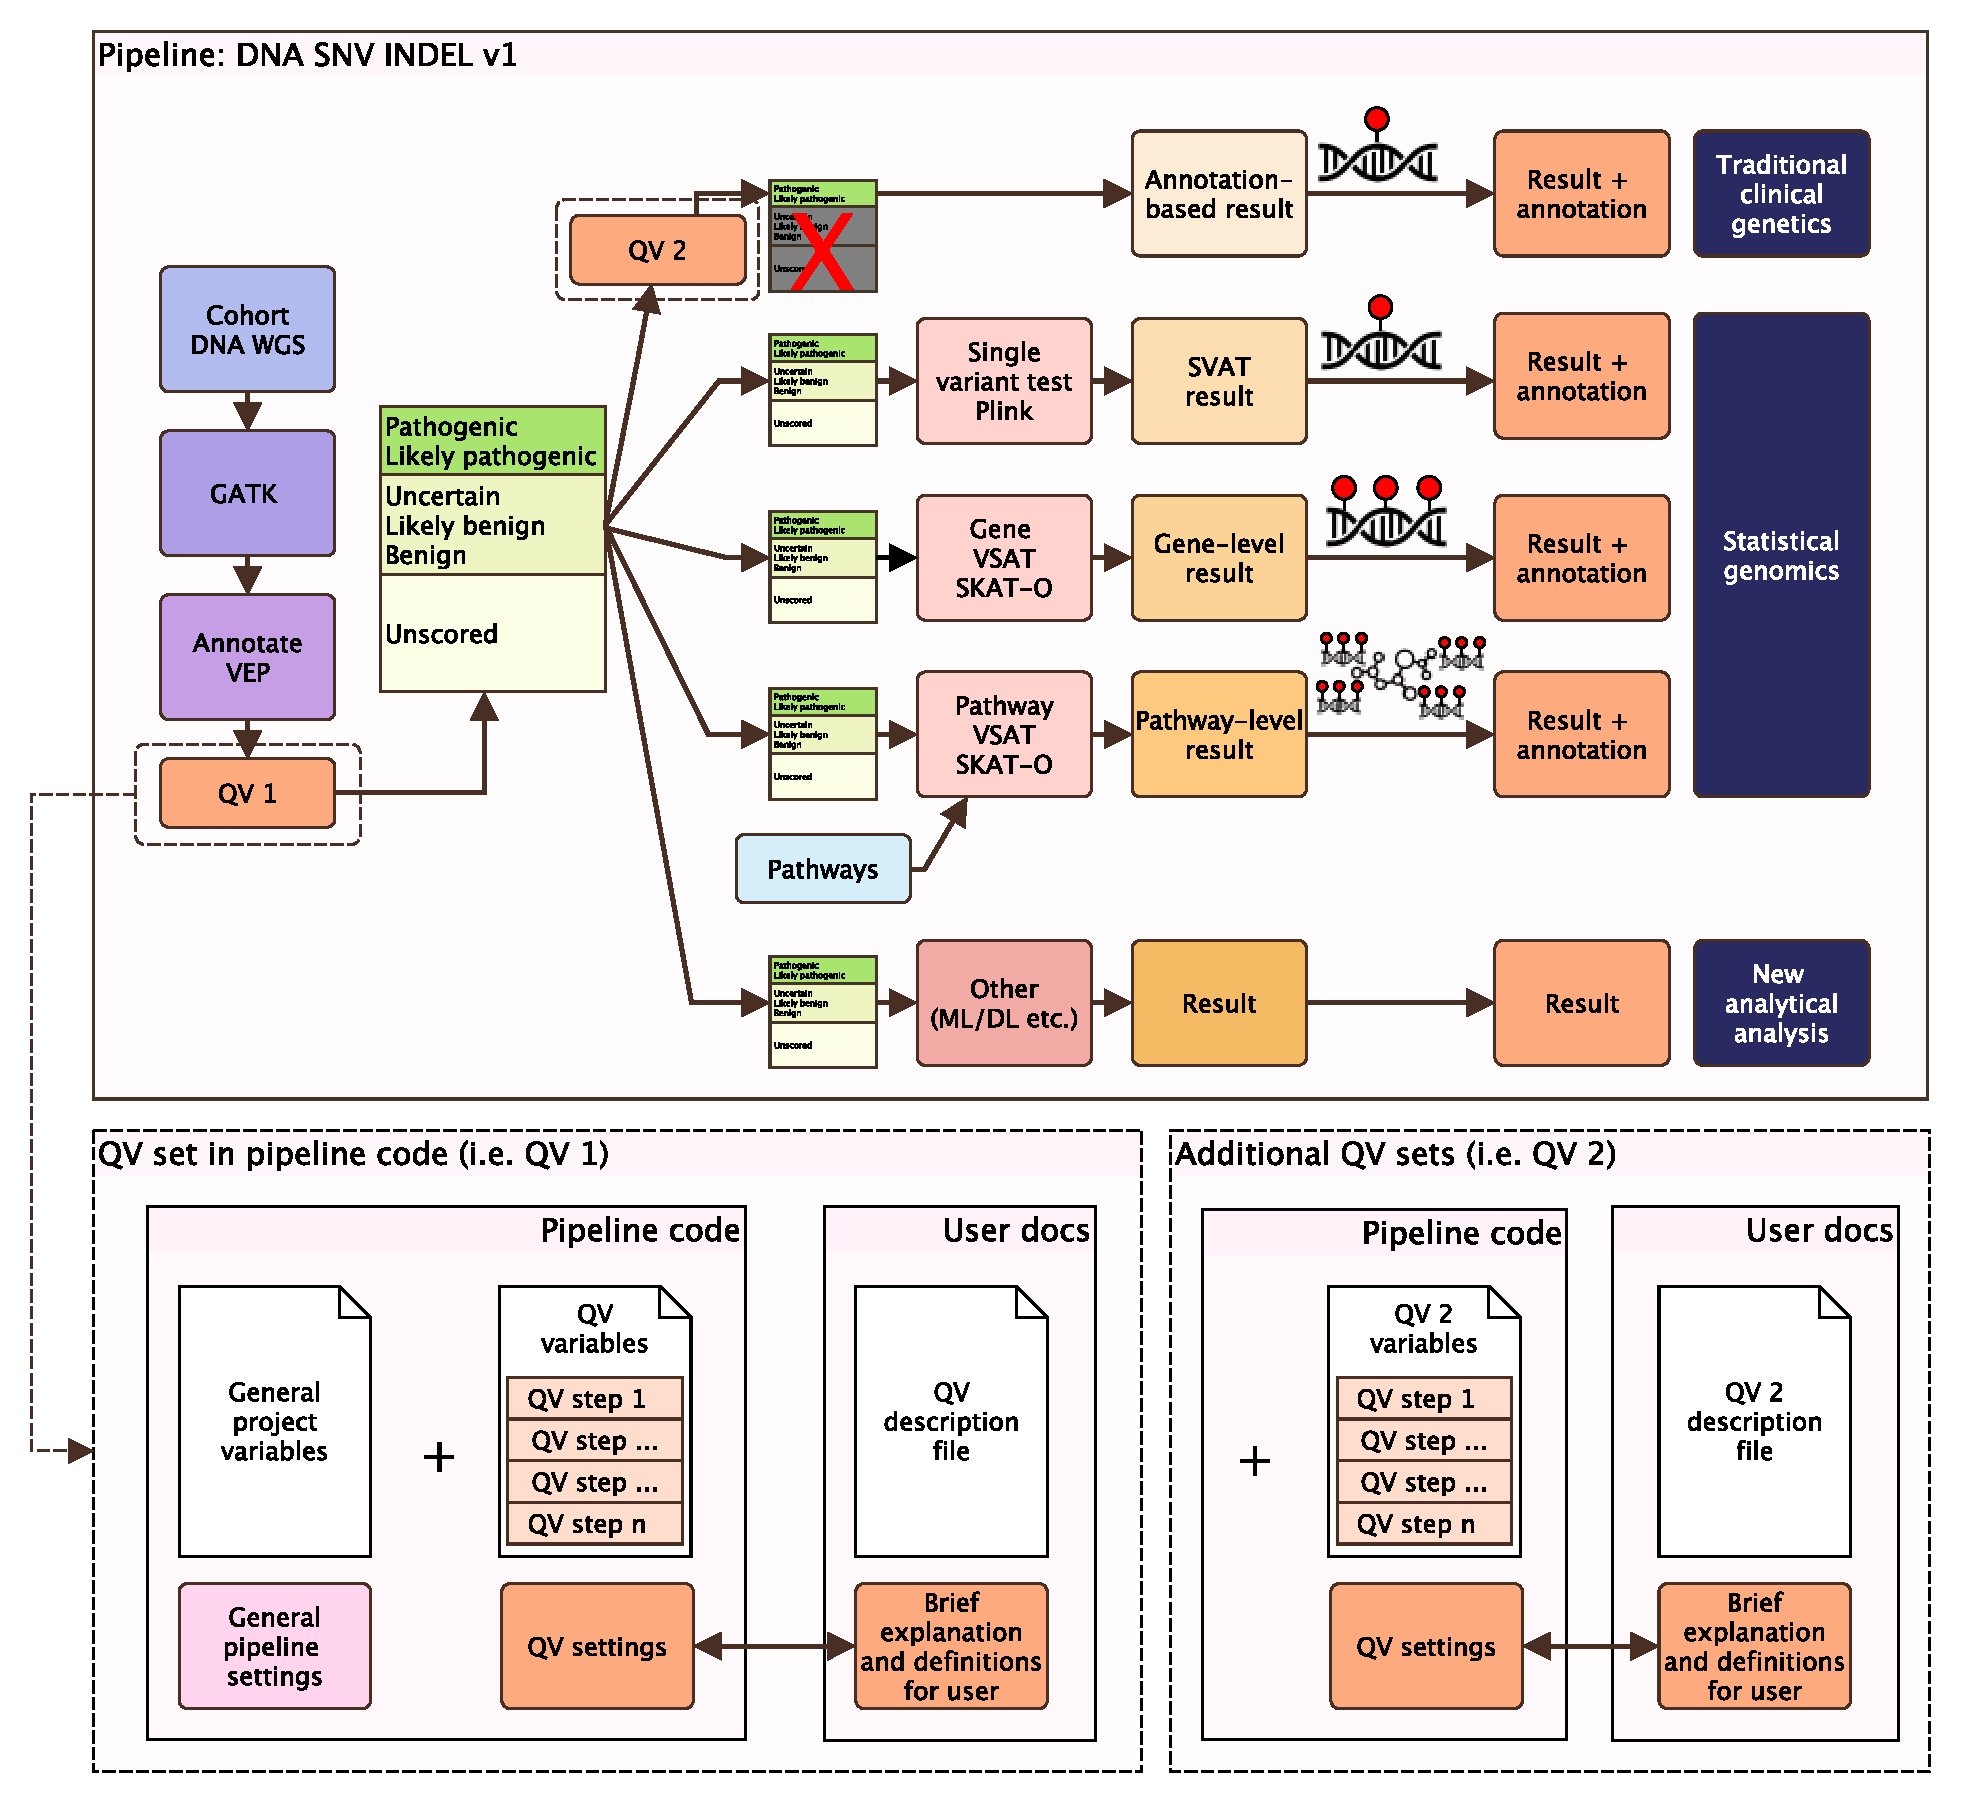
\includegraphics[width=\textwidth]{./images/qv_pipeline_with_file_vcurrent.pdf}
\end{minipage}\\[-2ex]
\begin{minipage}{0.9\textwidth}
\raggedright B\\[0.5ex]
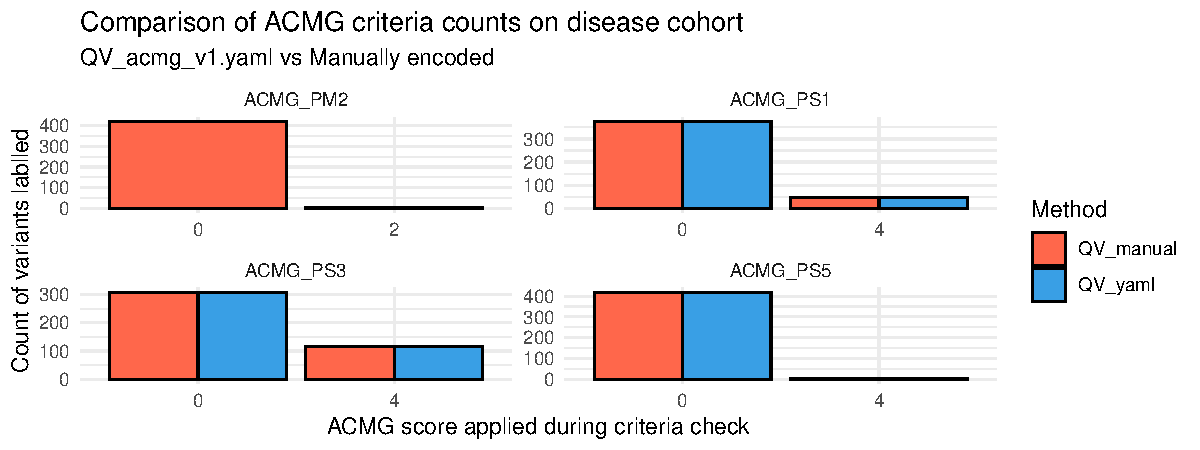
\includegraphics[width=\textwidth]{./images/Guru_singlecase_validation_of_yaml_vs_manual.pdf}
\end{minipage}
    \caption{Summary of the QV application for a WGS pipeline. In panel (A), \ac{qv}1 and \ac{qv}2 are presented as sequentially piped protocol steps. In this example, \ac{qv}2 differs from \ac{qv}1 by retaining only likely/pathogenic variants (indicated by a red X). The QV file loaded by the analysis pipeline comprise a description field (optional) and a variables field (mandatory). The \ac{qv} criteria may be spread throughout the pipeline.
    (B) Validation case study using an \ac{acmg} criteria subset, demonstrating a 100\% match between manually encoded and standardised YAML-based methods (\texttt{qv\_files/acmg\_criteria.yaml}) for assigning pathogenicity scores.}
    \label{fig:qv_pipeline_with_file_vcurrent_guru_case_study_result}
\end{figure}
%\begin{figure}[h!]
%    \centering
%   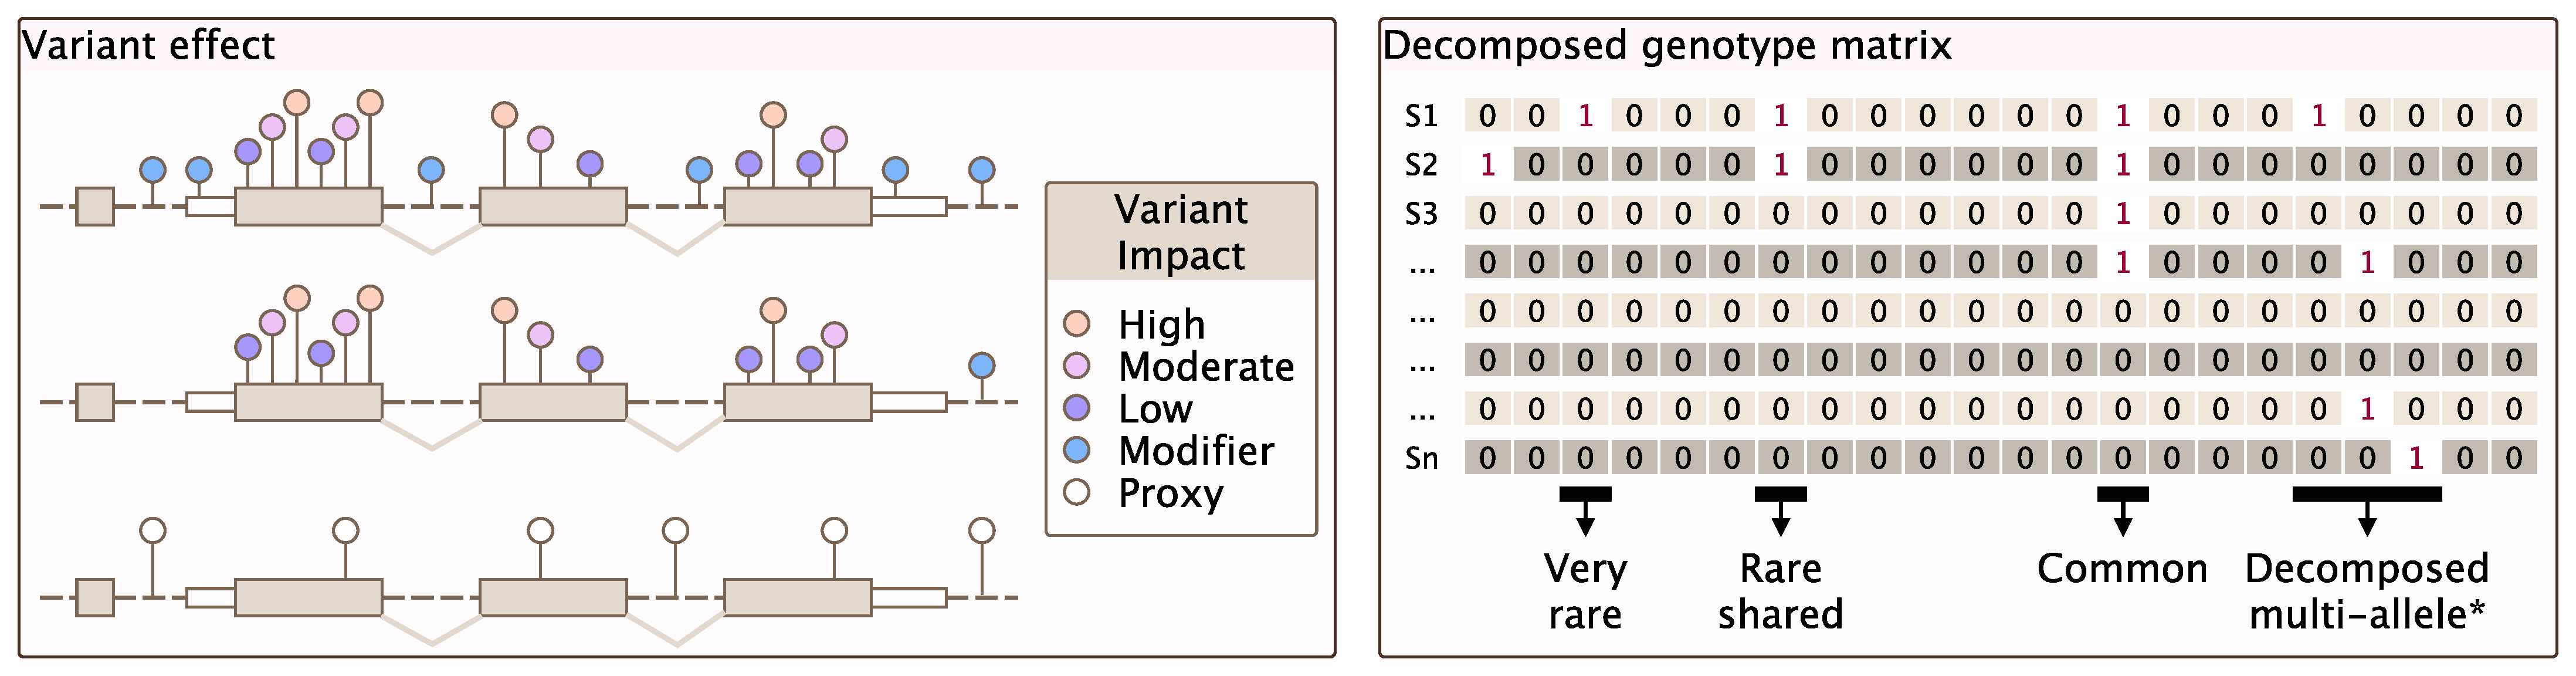
\includegraphics[width=0.8\textwidth]{./images/candidate_variants_effect_to_matrix_pink.pdf}
%      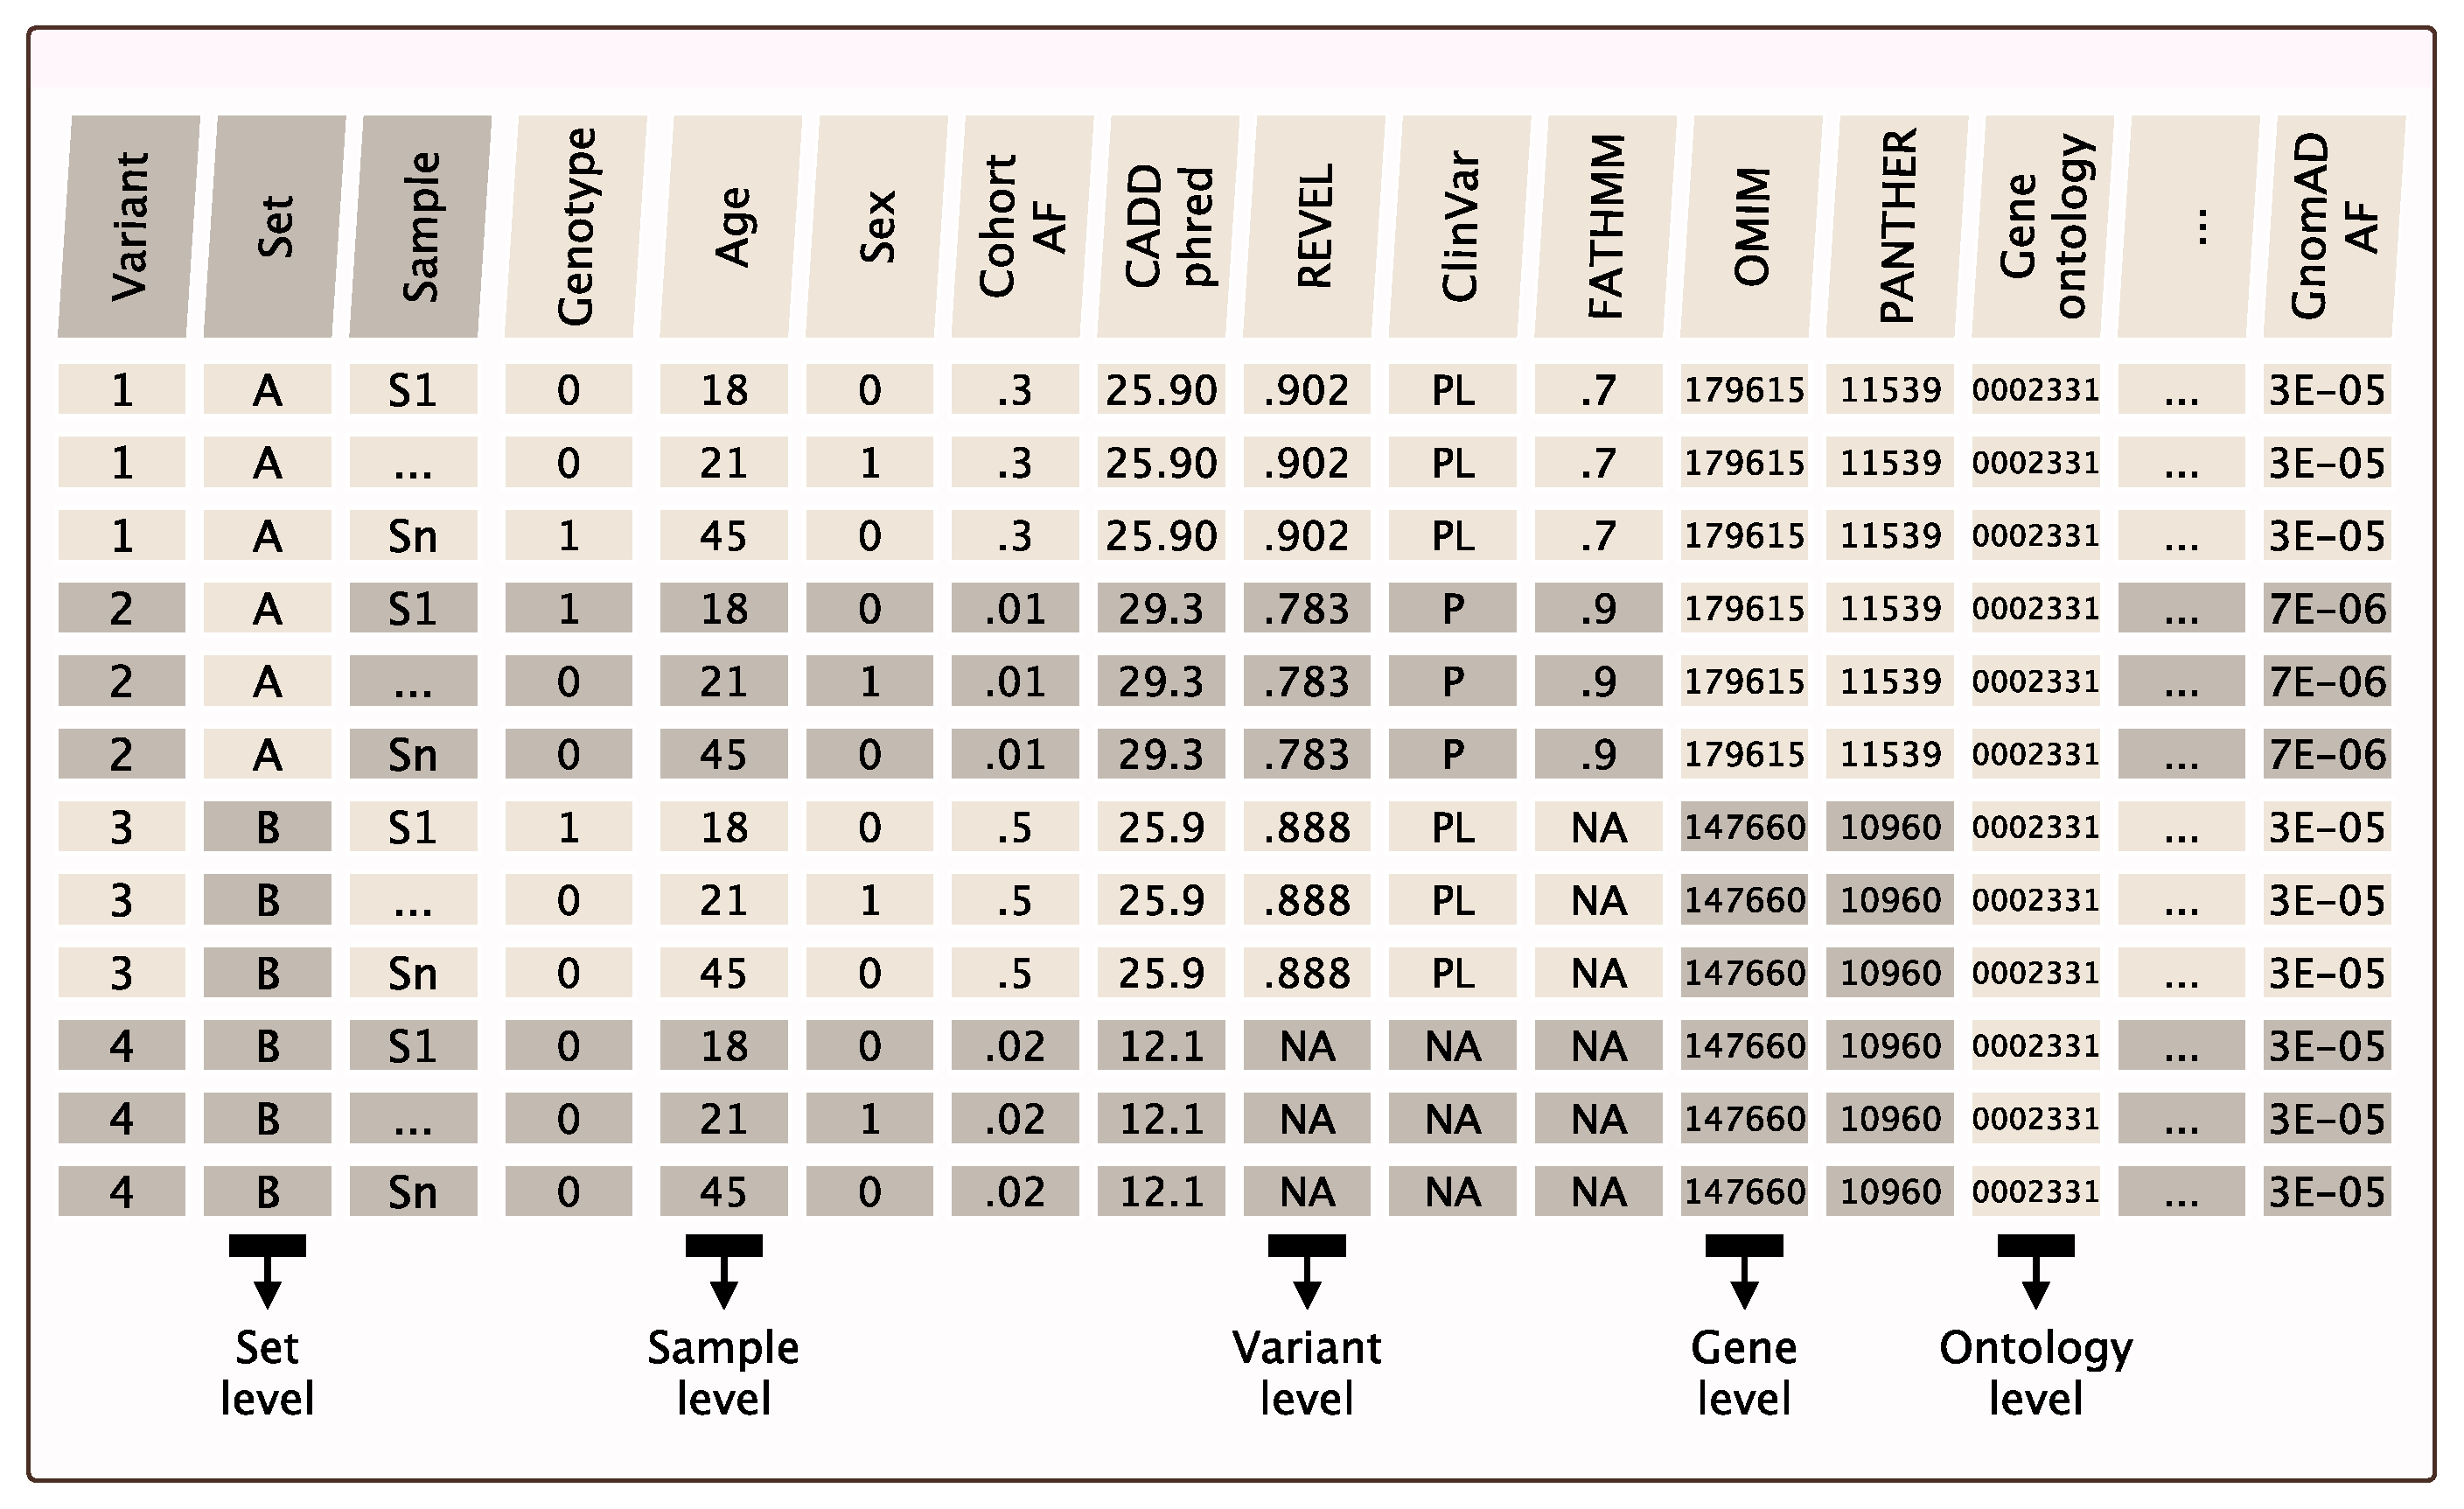
\includegraphics[width=0.8\textwidth]{./images/candidate_variants_sequence_annotation_pink.pdf}
%    \caption{
%Top: 
%    }
%        \label{fig:candidate_variants_sequence_annotation}
%\end{figure}

\FloatBarrier
\section{Methods}
\subsection{Implementation} \label{sec:framework}

By introducing a new vocabulary and a standard reference model for \ac{qv}s, we aim to clarify the concept and improve communication and methodological discussion across disciplines for more advanced tasks.
Implementation configurations and roles within analysis pipelines include, for example:
theoretical pipelining of \ac{qv} sets,
establishing public or standardised \ac{qv} sets for specific analytical scenarios, and 
recognition that \ac{qv}s are integral throughout the analysis pipeline rather than confined to a single end-stage

We introduce a simple framework for the effective use of \ac{qv} protocols, comprising four components as illustrated in \textbf{Figure \ref{fig:qv_pipeline_with_file_vcurrent_guru_case_study_result} (A)}:

\begin{itemize}
    \item \textbf{1. Variables}: The criteria variables sourced as part of the pipeline (see \textbf{Box \ref{box:acmg_criteria_yaml}}).
    \item \textbf{2a. Technical description}: An optional narrative detailing each step within the overall \ac{qv} set (see \textbf{Box \ref{box:acmg_criteria_yaml}}).
    \item \textbf{2b. \ac{ppi} description}: An optional narrative providing a patient-focused interpretation of the protocol, incorporating preferences and priorities.
    \item \textbf{3. \ac{qv} set ID}: A unique identifier that links analysis records.
    \item \textbf{4. Source code}: The implementation of the variables file within the pipeline code, for example through custom scripts or workflow managers.
\end{itemize}

We also propose the \ac{qv} set ID as a unique identifier linking variant sets used in analyses. This facilitates integration into databases,
by representing data in formats such as \ac{rdf} schemas \cite{toure2023fairification}, and allows for features including \ac{sha256} hash functions, \ac{uuid}s, semantic combinations, \ac{iri} incorporation, registry-based allocation, and standard mapping such as \ac{snomedct}. The results can be used alongside other genomic-specific concepts spanning from sample processing to the sequencing run \cite{van2023bridging}.

This framework efficiently manages \ac{qv}-specific variables (e.g. allele frequency thresholds) separately from general pipeline settings, ensuring clarity and specificity. Its versatile format supports applications across genomic analyses and by linking the \ac{qv} set ID to both results and raw data sources in a database for downstream interpretation and reporting.

\subsection{Example application of qualifying variants in WGS analysis}

Multiple \ac{qv} protocols can be combined to generate progressively filtered datasets tailored to specific analytical needs. Often, different \ac{qv} sets are applied sequentially, with the final outcomes merged to address distinct objectives. For instance, a comprehensive analysis pipeline might integrate:
\begin{itemize}
  \item \colorbox{kispiblue!05}{\texttt{QV SNV/INDEL}}  \ac{snvindel},
  \item \colorbox{kispiblue!05}{\texttt{QV CNV}} \ac{cnv},
  \item \colorbox{kispiblue!05}{\texttt{QV structural variation}},
  \item \colorbox{kispiblue!05}{\texttt{QV rare disease known}}, and 
  \item \colorbox{kispiblue!05}{\texttt{QV statistical association \ac{qc}}}.
\end{itemize}
The final analysis yields (1) a joint cohort disease association (e.g. variant P-values) and (2) individual single-case results (e.g. clinical genetics diagnosis for a patient)
\cite{auwera_genomics_2020, li2025statistical}.
As an example, in 
\textbf{Figure \ref{fig:qv_pipeline_with_file_vcurrent_guru_case_study_result} (A)}
we focus on a SNV/INDEL pipeline employing two \ac{qv} sets:
\colorbox{colorSUNSET2!20}{\texttt{QV SNV INDEL 1}} for flexible cohort-level filtering, and 
\colorbox{colorSUNSET2!20}{\texttt{QV SNV INDEL 2}} for stricter filtering in subsequent single-case analysis. The pipeline is illustrated in \textbf{Box \ref{box:pipe}}, and can be summarised as follows:

``A cohort of patient WGS data was analysed to identify genetic determinants for phenotype X. Initially, a flexible \ac{qv} set was applied using the 
\colorbox{colorSUNSET1!10}{\texttt{pipeline DNA SNV INDEL v1}}, which implements the \colorbox{colorSUNSET2!20}{\texttt{QV SNV INDEL 1}} criteria to produce the prepared dataset (\colorbox{colorSUNSET3!10}{\texttt{dataset DNA SNV INDEL v1}}). This dataset was then analysed alongside other modules (e.g. \colorbox{colorSUNSET4!10}{\texttt{PCA SNV INDEL v1}} and \colorbox{colorSUNSET5!10}{\texttt{statistical genomics v1}}) to derive a cohort-level association signal (Result 1). Next, the same prepared dataset was re-filtered with the stricter \colorbox{colorSUNSET2!20}{\texttt{QV SNV INDEL 2}} criteria to identify known causal variants for each patient, yielding the final dataset (\colorbox{colorSUNSET3!10}{\texttt{dataset DNA SNV INDEL v2}}) and resulting in individual case reports (Result 2).''

\begin{tcolorbox}[
    colback=white!0,
    colframe=black,
    boxrule=1pt,
    arc=1mm,
    outer arc=1mm,
    title=\textbf{\refstepcounter{myboxcounter}\label{box:pipe}Box \themyboxcounter: Example diagrammatic representation}
]
\dirtree{%
.1 \colorbox{colorSUNSET1!10}{\texttt{pipeline DNA SNV INDEL v1}}.
.2 Flexible \ac{qv} criteria.
.3 \colorbox{colorSUNSET2!20}{\texttt{QV SNV INDEL 1}} $\rightarrow$ \colorbox{colorSUNSET3!10}{\texttt{dataset DNA SNV INDEL v1}}.
.4 \colorbox{colorSUNSET4!10}{\texttt{PCA SNV INDEL v1}}.
.4 \colorbox{colorSUNSET5!10}{\texttt{statistical genomics v1}} $\rightarrow$ Result 1.
.3 \colorbox{colorSUNSET3!10}{\texttt{dataset DNA SNV INDEL v1}}.
.4 Rare disease \ac{qv} criteria.
.5 \colorbox{colorSUNSET2!20}{\texttt{QV SNV INDEL 2}} $\rightarrow$ \colorbox{colorSUNSET3!10}{\texttt{dataset DNA SNV INDEL v2}}.
.6 \colorbox{colorSUNSET5!10}{\texttt{single case report SNV INDEL v1}} $\rightarrow$ Result 2.
.3 Joint analysis output.
}
\medskip

Joint analysis output from:\\
Result 1 = Cohort-level association signal (e.g. variant P-value).\\
Result 2 = Single variant report per patient.
\end{tcolorbox}


\subsection{Usage in a Validation Study}

In the following validation study, we demonstrate that standardised \ac{qv} criteria achieve a 100\% match in criterion application when compared to the conventional manual approach. This analysis was performed on an in-house rare disease cohort of 940 individuals, which had been pre-processed for \ac{qc} and filtered using a minimal \ac{qv} test set.
%, as described previously.
Initially, we implemented an \ac{acmg} variant classification protocol \cite{richards2015standards} manually. We then re-implemented the same protocol using the new standardised \ac{qv} criteria in YAML format. Our findings confirm that both methods produce identical results.

We used genome-wide set of variants which was filtering to target rare varaints (\ac{maf} $< 0.01$) restricted to known disease genes based on the Genomics England panel ``Primary immunodeficiency or monogenic inflammatory bowel disease,'' retrieved using our PanelAppRex R repository (\url{https://github.com/DylanLawless/PanelAppRex}) 
\cite{lawless_panelapprex_2025}. 
This provided us with 6026 candidate variants annotated with 376 information sources.

The annotation interpretation dataset was prepared in R using GuRu, our variant interpretation tool that consolidates all annotation sources and scores variants as candidate causal. The dataset was imported from gVCF format as output by \ac{vep}.
% A subset of key annotations used for \ac{qv} is illustrated in \textbf{Figure \ref{fig:qv_pipeline_with_file_vcurrent_guru_case_study_result}}.

We selected the first eight \ac{acmg} criteria for assigning pathogenicity scores to variants \cite{richards2015standards}; six of these were relevant for this cohort. First, the analysis was performed manually by hard-coding each criterion in the pipeline script, reflecting a typical workflow. Second, the same criteria were imported from the \ac{qv} YAML file for the new standardised approach. The outputs from both methods were captured and compared.
The \ac{qv} criteria were provided in YAML format in the file \texttt{qv\_files/acmg\_criteria.yaml} 
(see \textbf{Box \ref{box:acmg_criteria_yaml}}).

Additional details of the YAML criteria in this \ac{qv} set include definitions for \texttt{ACMG\_PS1} (identifying previously established pathogenic amino acid changes), \texttt{ACMG\_PS3} (supporting functional studies with matching inheritance patterns), and \texttt{ACMG\_PS5} (covering compound heterozygosity with high-impact variants). The criteria for \texttt{ACMG\_PM2} and \texttt{ACMG\_PM3} assess variant frequency and in trans occurrences, respectively, while \texttt{PS2} and \texttt{PS4} were not applicable to this cohort.

Individual steps within the \ac{qv} criteria can be further classified for organisational purposes using simple labels such as ``QC'' and ``filter''. For example, filtering thresholds (e.g. allele frequency > 0.1 in a cohort, < 0.1 in gnomAD) may be applied directly to exclude variants, while annotation-based criteria (e.g. QC flags) might not remove variants outright but instead inform downstream analyses that integrate multiple \ac{qv} filters.

\begin{tcolorbox}[
    colback=white!0,
    colframe=black,
    boxrule=1pt,
    arc=1mm,
    outer arc=1mm,
    title=\textbf{\refstepcounter{myboxcounter}\label{box:acmg_criteria_yaml}Box \themyboxcounter: qv\_files/acmg\_criteria.yaml}
]
\begin{verbatim}
qv_set_id: acmg_sf_v3.2

acmg_pvs1:
  description_technical: >
    Null variants (IMPACT = HIGH) in genes where 
    loss-of-function causes disease.
    Includes homozygous variants, dominant inheritance, 
    and compound heterozygous cases.
    Compound heterozygosity is considered when both 
    variants are HIGH impact. WARNING: Not phase checked.
  logic: "or"
  conditions:
    - condition:
        field: IMPACT
        value: "HIGH"
        operator: "=="
...
shasum -a 256 acmg_criteria.yaml | fold -w 32
d91fde41a5fff48631adecba38773d61
9ae8cd5cff9b9b42ef7f5efbd6bbfcdf
acmg_criteria.yaml
\end{verbatim}
\end{tcolorbox}


\section{Results}
\subsection{Validation Case Study}

We validated our \ac{qv} protocol using \ac{acmg}-based criteria for a rare disease cohort of 940 individuals. 
We then conducted the variant classification using two approaches: a conventional manual method with hard-coded criteria, and our new YAML-based implementation
As shown in \textbf{Figure \ref{fig:qv_pipeline_with_file_vcurrent_guru_case_study_result} (B)}, 
the outputs from both methods were identical, demonstrating a 100\% match. This confirms that our standardised, shareable \ac{qv} criteria can be imported and applied programmatically with equivalent accuracy, providing a reproducible resource that is adaptable across different pipelines and programming environments.
%Figure~\ref{fig:guru_case_study_guruscores} illustrates 
The final annotation results in this pipeline allow for automated retrieval of top candidate pathogenic variants using \ac{acmg} scoring methods \cite{richards2015standards, tavtigian2020fitting}.

\section{Summary}
This paper introduces a standardised framework for integrating qualifying variants into genomic analysis pipelines, enhancing reproducibility, interpretability and the seamless translation of research findings into clinical practice.

\section{Funding}
This project was supported through the grant NDS-2021-911 (SwissPedHealth) from the Swiss Personalized Health Network and the Strategic Focal Area 'Personalized Health and Related Technologies' of the ETH Domain (Swiss Federal Institutes of Technology).

\section{Acknowledgements}
Acknowledgements We would like to thank all the patients and families who have been providing advice on SwissPedHealth and its projects, as well as the clinical and research teams at the participating institutions.

\section{Contributions}
DL designed the work and contributed to the manuscript.
AS, SB, VS, DH, SÖ, JA contributed to the manuscript.
JF, SF, LJS supervised the work, manuscript, and applied for funding.

\section{Competing interests}
None declared.

%\section{Collaborators}
%The SwissPedHealth consortium may be named here for publication and is prepared as a comment in the LaTeX document.
% SwissPedHealth consortium: Andrea Agostini (Department of Computer Science, Institute for Machine Learning, ETH Zurich, Zurich, Switzerland), Anita Rauch (Institute of Medical Genetics, University of Zurich, Zurich, Switzerland), Anna Hartung (Inselspital, Bern University Hospital, University of Bern, Switzerland), Audrey van Drogen (PHRT Swiss Multi-Omics Centre [SMOC], ETH Zurich, Zurich, Switzerland \& Institute of Translational Medicine [ITM], Department of Health Sciences and Technology [D-HEST], ETH Zurich, Zurich, Switzerland), Aurélie Martin Necker (Patient and Family Advisory Committee, SwissPedHealth), Ben D Spycher (Institute of Social and Preventive Medicine [ISPM], University of Bern, Bern, Switzerland), Christian Kahlert (Ostschweizer Kinderspital, St Gallen, Switzerland), Christopher B Forrest (Center for Applied Clinical Research, Children’s Hospital of Philadelphia, Philadelphia, USA), Claudia E Kuehni (Institute of Social and Preventive Medicine [ISPM], University of Bern, Bern, Switzerland \& Division of Paediatric Respiratory Medicine and Allergology, Children's University Hospital, Inselspital, University of Bern, Bern, Switzerland), Cornelia Hagman (Department of Intensive Care and Neonatology and Children’s Research Centre, University Children’s Hospital Zurich, University of Zurich, Zurich, Switzerland), D Sean Froese (Division of Metabolism and Children’s Research Centre, University Children’s Hospital Zurich, University of Zurich, Zurich, Switzerland), Daphné Chopard (Department of Computer Science, Institute for Machine Learning, ETH Zurich, Zurich, Switzerland \& Department of Intensive Care and Neonatology and Children’s Research Centre, University Children’s Hospital Zurich, University of Zurich, Zurich, Switzerland), Dylan Lawless (School of Life Sciences, Ecole Polytechnique Fédérale de Lausanne, Lausanne, Switzerland \& Department of Intensive Care and Neonatology and Children’s Research Centre, University Children’s Hospital Zurich, University of Zurich, Zurich, Switzerland), Effy Vayena (Department of Health Sciences and Technology, Institute of Translational Medicine, ETH Zurich, Zurich, Switzerland), Eirini I Petrou (Department of Health Sciences and Technology, Institute of Translational Medicine, ETH Zurich, Zurich, Switzerland), Emanuele Palumbo (Department of Computer Science, Institute for Machine Learning, ETH Zurich, Zurich, Switzerland), Eric Giannoni (Clinic of Neonatology, Lausanne University Hospital, University of Lausanne, Lausanne, Switzerland), Fabiën N Belle (Institute of Social and Preventive Medicine [ISPM], University of Bern, Bern, Switzerland), Ioannis Xenarios (PHRT Swiss Multi-Omics Centre [SMOC], EPFL, Lausanne, Switzerland \& Department of Computational Biology, University of Lausanne, Lausanne, Switzerland \& Health 2030 Genome Center, Foundation Campus Biotech, Geneva, Switzerland), Jacques Fellay (School of Life Sciences, Ecole Polytechnique Fédérale de Lausanne, Lausanne, Switzerland \& Biomedical Data Science Center, Lausanne University Hospital, University of Lausanne, Lausanne, Switzerland), Jana Pachlopnik Schmid (Division of Immunology and Children’s Research Centre, University Children’s Hospital Zurich, University of Zurich, Zurich, Switzerland), Julia A Bielicki (Paediatric Research Center, University Children's Hospital Basel [UKBB], University of Basel, Basel, Switzerland \\& Centre for Neonatal and Paediatric Infection, St George’s, University of London, London, UK), Julia E Vogt (Department of Computer Science, Institute for Machine Learning, ETH Zurich, Zurich, Switzerland), Kathrin Hofmann (Patient and Family Advisory Committee, SwissPedHealth), Katrin Männik (PHRT Swiss Multi-Omics Centre [SMOC], EPFL, Lausanne, Switzerland \\& Center for Integrative Genomics, University of Lausanne, Lausanne, Switzerland \& Health 2030 Genome Center, Foundation Campus Biotech, Geneva, Switzerland), Keith Harshman (PHRT Swiss Multi-Omics Centre [SMOC], EPFL, Lausanne, Switzerland \& Health 2030 Genome Center, Foundation Campus Biotech, Geneva, Switzerland), Kelly Ormond (Department of Health Sciences and Technology, Institute of Translational Medicine, ETH Zurich, Zurich, Switzerland \& Department of Genetics, Stanford University School of Medicine, Stanford, California, USA), Klara Posfay-Barbe (Hôpitaux Universitaires de Genève, Geneva, Switzerland), Léa Ho Dac (Division of Paediatric Respiratory Medicine and Allergology, Department of Paediatrics, Inselspital, Bern University Hospital, University of Bern, Switzerland), Lorenz M Leuenberger (Institute of Social and Preventive Medicine [ISPM], University of Bern, Bern, Switzerland), Luregn J Schlapbach (Department of Intensive Care and Neonatology and Children’s Research Centre, University Children’s Hospital Zurich, University of Zurich, Zurich, Switzerland \& Child Health Research Centre, The University of Queensland, Brisbane, Australia), Manon Jaboyedoff (Pediatric Infectious Diseases and Vaccinology Unit, Service of Pediatrics, Department Mother-Woman-Child, Lausanne University Hospital and University of Lausanne, Lausanne, Switzerland), Mariam Ait Oumelloul (School of Life Sciences, Ecole Polytechnique Fédérale de Lausanne, Lausanne, Switzerland), Martin Stocker (Luzerner Kantonsspital, Luzern, Switzerland), Matthias R Baumgartner (Division of Metabolism and Children’s Research Centre, University Children’s Hospital Zurich, University of Zurich, Zurich, Switzerland), Nicola Zamboni (PHRT Swiss Multi-Omics Centre [SMOC], ETH Zurich, Zurich \& Institute of Molecular Systems Biology, ETH Zurich, Zurich, Switzerland), Nicole Goebel (Research and Analyses Services, Digitalisation \& ICT Division, University Hospital Basel, Basel, Switzerland), Patrick G A Pedrioli (PHRT Swiss Multi-Omics Centre [SMOC], ETH Zurich, Zurich, Switzerland \& Institute of Translational Medicine [ITM], Department of Health Sciences and Technology [D-HEST], ETH Zurich, Zurich, Switzerland \& Swiss Institute of Bioinformatics, Lausanne, Switzerland \& Department of Biology, Institute of Molecular Systems Biology, Swiss Federal Institute of Technology/ETH Zürich, Zurich, Switzerland), Philipp Latzin (Division of Paediatric Respiratory Medicine and Allergology, Department of Paediatrics, Inselspital, Bern University Hospital, University of Bern, Switzerland), Rebeca Mozun (Department of Intensive Care and Neonatology and Children’s Research Centre, University Children’s Hospital Zurich, University of Zurich, Zurich, Switzerland), Roger Lauener (Ostschweizer Kinderspital, St Gallen, Switzerland), Sandra Goetze (PHRT Swiss Multi-Omics Centre [SMOC], ETH Zurich, Zurich, Switzerland \& Institute of Translational Medicine [ITM], Department of Health Sciences and Technology [D-HEST], ETH Zurich, Zurich, Switzerland), Seraina Prader (Division of Immunology and Children’s Research Centre, University Children’s Hospital Zurich), Simon Boutry (School of Life Sciences, Ecole Polytechnique Fédérale de Lausanne, Lausanne, Switzerland), Sven Schulzke (Department of Neonatology, University Children's Hospital Basel [UKBB], University of Basel, Basel, Switzerland), Tatjana Welzel (Paediatric Research Center, University Children's Hospital Basel [UKBB], University of Basel, Basel, Switzerland), Thomas M Sutter (Department of Computer Science, Institute for Machine Learning, ETH Zurich, Zurich, Switzerland), Varvara Dimopoulou (Clinic of Neonatology, Lausanne University Hospital and University of Lausanne, Lausanne, Switzerland), Vito RT Zanotelli (Division of Metabolism and Children’s Research Centre, University Children’s Hospital Zurich, University of Zurich, Zurich, Switzerland), Xeni Deligianni (Research and Analyses Services, Digitalisation \& ICT Division, University Hospital Basel, Basel, Switzerland), Xenia Bovermann (Division of Paediatric Respiratory Medicine and Allergology, Department of Paediatrics, Inselspital, Bern University Hospital, University of Bern, Switzerland), Yara Shoman (Institute of Social and Preventive Medicine [ISPM], University of Bern, Bern, Switzerland).

\clearpage
\bibliographystyle{unsrtnat}
\bibliography{references} 

\end{document}
